\bookchapter{Pythagoras and the distance formula}\label{ch:pythagoras}

\section*{Pythagoras' theorem}
In a right triangle with legs $a$ and $b$ and hypotenuse $c$:
\[
a^2+b^2=c^2.
\]
Geometrically: the area of the square on the hypotenuse equals the sum of the areas of the squares on the two legs.

\begin{center}
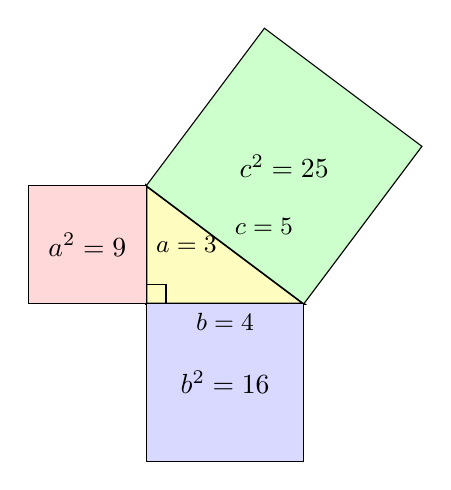
\begin{tikzpicture}[scale=0.5]
  \filldraw[fill=yellow!25,draw=black,thick] (0,0) -- (4,0) -- (0,3) -- cycle;
  \filldraw[fill=blue!15,draw=black] (0,0) -- (4,0) -- (4,-4) -- (0,-4) -- cycle;
  \filldraw[fill=red!15,draw=black] (0,0) -- (0,3) -- (-3,3) -- (-3,0) -- cycle;
  \filldraw[fill=green!20,draw=black] (4,0) -- (0,3) -- (3,7) -- (7,4) -- cycle;
  \draw (0.5,0) -- (0.5,0.5) -- (0,0.5);
  \node at (2,-2) {$b^2=16$};
  \node at (-1.5,1.5) {$a^2=9$};
  \node at (3.5,3.5) {$c^2=25$};
  \node[above right,font=\small] at (2,1.5) {$c=5$};
  \node[below,font=\small] at (2,0) {$b=4$};
  \node[right,font=\small] at (0,1.5) {$a=3$};
\end{tikzpicture}

\small\textbf{Figure 9.} The squares on the legs ($9+16$) have together the same area as the square on the hypotenuse ($25$).
\end{center}

\begin{example}
Legs $6$ and $8$: $c=\sqrt{36+64}=10$. A leg from hypotenuse $13$ and leg $5$: $b=\sqrt{169-25}=12$. The converse also holds: a triangle with sides $a,b,c$ and $a^2+b^2=c^2$ has a right angle.
\end{example}

\section*{Distance between two points}
The distance between $P_1=(x_1,y_1)$ and $P_2=(x_2,y_2)$ is the hypotenuse of a right triangle with legs $\Delta x=x_2-x_1$ and $\Delta y=y_2-y_1$:
\[
d=\sqrt{(x_2-x_1)^2+(y_2-y_1)^2}.
\]

\begin{center}
\begin{tikzpicture}[>=Stealth, scale=0.8]
  \draw[gray!40,very thin] (0,0) grid (7,5);
  \draw[->] (0,0) -- (7.4,0) node[right]{$x$};
  \draw[->] (0,0) -- (0,5.4) node[above]{$y$};
  \foreach \x in {1,...,7} \node[below,font=\scriptsize] at (\x,0) {$\x$};
  \foreach \y in {1,...,5} \node[left,font=\scriptsize] at (0,\y) {$\y$};
  \draw[dashed,thick,gray] (1,1) -- (5,1) node[midway,below]{$\Delta x=4$} -- (5,4) node[midway,right]{$\Delta y=3$};
  \draw[very thick,blue] (1,1) -- (5,4) node[midway,above left]{$d=5$};
  \fill[red] (1,1) circle (2.5pt) node[above left]{$P_1(1,1)$};
  \fill[red] (5,4) circle (2.5pt) node[above right]{$P_2(5,4)$};
\end{tikzpicture}

\small\textbf{Figure 10.} The distance is the hypotenuse of the triangle formed by $\Delta x$ and $\Delta y$.
\end{center}

\begin{example}
A robot at $(1,2)$ sees a ball at $(7,10)$. The distance is $\sqrt{6^2+8^2}=\sqrt{100}=10$.
\end{example}

In three dimensions we apply Pythagoras twice and get
\[
d=\sqrt{(x_2-x_1)^2+(y_2-y_1)^2+(z_2-z_1)^2}.
\]

\begin{center}
\begin{tikzpicture}[x={(-0.45cm,-0.33cm)}, y={(0.75cm,0cm)}, z={(0cm,0.5cm)}, >=Stealth]
  \draw[gray,dashed] (0,3,0) -- (2,3,0);
  \draw[gray,dashed] (0,3,0) -- (0,0,0);
  \draw[gray,dashed] (0,3,0) -- (0,3,6);
  \draw[thick] (2,0,0) -- (2,3,0) -- (2,3,6) -- (2,0,6) -- cycle;
  \draw[thick] (0,0,0) -- (2,0,0);
  \draw[thick] (0,0,6) -- (2,0,6);
  \draw[thick] (0,0,0) -- (0,0,6);
  \draw[thick] (0,3,6) -- (2,3,6);
  \draw[thick] (0,0,6) -- (0,3,6);
  \draw[red,very thick] (2,0,0) -- (0,3,6);
  \node[below left,font=\small] at (1,0,0) {$2$};
  \node[below,font=\small] at (2,1.5,0) {$3$};
  \node[right,font=\small] at (2,3,3) {$6$};
  \node[red,above,font=\small] at (1,1.5,3) {$d=7$};
\end{tikzpicture}

\small\textbf{Figure 11.} The space diagonal of a box with edges $2$, $3$ and $6$ has length $d=\sqrt{4+9+36}=7$.
\end{center}

\section*{Other ways to measure ``how far off''}
The straight-line distance above is the \emph{Euclidean distance} ($L_2$). Sometimes the \emph{Manhattan distance} $|\Delta x|+|\Delta y|$ ($L_1$) is used, which measures the way along a street grid. In machine learning, the \emph{squared error} $\Delta x^2+\Delta y^2$ is the most common error measure because it avoids the square root and is easy to differentiate.

\begin{center}
\begin{tikzpicture}[>=Stealth, scale=0.9]
  \draw[gray!40,very thin] (0,0) grid (7,8);
  \draw[->] (0,0) -- (7.4,0) node[right]{$x$};
  \draw[->] (0,0) -- (0,8.4) node[above]{$y$};
  \draw[red,very thick] (2,3) -- (5,3) -- (5,7);
  \node[red,below] at (3.5,3) {$3$};
  \node[red,right] at (5,5) {$4$};
  \draw[blue,very thick] (2,3) -- (5,7) node[midway,above left]{$5$};
  \fill (2,3) circle (2.5pt) node[left]{predicted $(2,3)$};
  \fill (5,7) circle (2.5pt) node[above right]{true $(5,7)$};
\end{tikzpicture}

\small\textbf{Figure 12.} Euclidean distance $5$ (blue), Manhattan distance $3+4=7$ (red), squared error $3^2+4^2=25$.
\end{center}

\section*{Circles}
All points at distance $r$ from a centre $(a,b)$ satisfy $(x-a)^2+(y-b)^2=r^2$. Points with a smaller left side are \emph{inside} the circle.

\begin{example}[Sensor range]
A robot at $(3,2)$ detects objects within $4$ m. Is a ball at $(5,5)$ in range? Its distance is $\sqrt{2^2+3^2}=\sqrt{13}\approx3.61<4$, so yes. A ball at $(8,3)$ has distance $\sqrt{26}\approx5.10>4$, so no.
\end{example}

\begin{center}
\begin{tikzpicture}[>=Stealth, scale=0.62]
  \draw[gray!40,very thin] (-1,-2) grid (8,6);
  \draw[->] (-1,0) -- (8.4,0) node[right]{$x$};
  \draw[->] (0,-2) -- (0,6.4) node[above]{$y$};
  \draw[thick,dashed,blue,fill=blue!6] (3,2) circle (4);
  \fill[blue] (3,2) circle (3pt) node[below left]{robot $(3,2)$};
  \fill[green!50!black] (5,5) circle (3pt) node[above right]{in range};
  \fill[red] (8,3) circle (3pt) node[above]{out of range};
  \draw[<->,blue] (3,2) -- (3+2.828,2+2.828) node[midway,below right]{$r=4$};
\end{tikzpicture}

\small\textbf{Figure 13.} The circle $(x-3)^2+(y-2)^2=16$ is the sensor range of the robot.
\end{center}

\begin{aibox}
A neural network's training loss is a (squared) distance between its prediction and the true answer, only in many more dimensions: the formula is identical, with more terms under the square root. Distances are also used to decide which objects are close to a robot, and to compare images in nearest-neighbour methods.
\end{aibox}

\section*{Practice problems}
\begin{enumerate}[label=\textbf{\thechapter.\arabic*}]
  \item Find the missing side of the right triangle: (a) legs $6$ and $8$; (b) legs $5$ and $12$; (c) hypotenuse $15$ and one leg $9$.
  \item Compute the distance between $(-1,2)$ and $(4,14)$.
  \item A robot at $(2,3)$ sees a ball at $(8,11)$. How far is it, and how far in the $x$- and $y$-direction?
  \item Compute the distance between $(1,2,3)$ and $(3,6,7)$.
  \item Is the point $(4,7)$ inside, on, or outside the circle with centre $(1,3)$ and radius $5$?
  \item A predicted position is $(1,2)$ and the true position is $(4,6)$. Compute the Euclidean distance, the Manhattan distance and the squared error.
  \item Does a triangle with sides $7$, $24$ and $25$ have a right angle?
  \item $\star$ A $5$ m ladder leans against a vertical wall, with its foot $3$ m from the wall. How high does it reach? If the foot is pulled out to $4$ m from the wall, how far does the top slide down?
  \item $\star$ Show that the 3D distance formula follows from applying Pythagoras twice.
\end{enumerate}

% =====================================================
